\documentclass[12pt,fleqn]{article}\usepackage{../../common}
\begin{document}
Genel Makroekonomi

Paranın Miktar Teorisi (Quantity Theory of Money) 

Bir liranın günlük hayat içinde dolaşımını düşünelim. Ben gidiyorum mesela
köşe başındaki satıcıdan bir poğaça alıyorum. Bu satıcı lirayı kızına
veriyor, kızı da onu lunaparkta ata binmek için kullanıyor. Atı kiralayan
Ali lirayı eve götürüyor, bir süre koltuk altında kaybediyor, tekrar
buluyor, sonra onu kahve almak için kullanıyor. Bütün bir sene içinde bu
lira üç kere harcanmış oluyor.

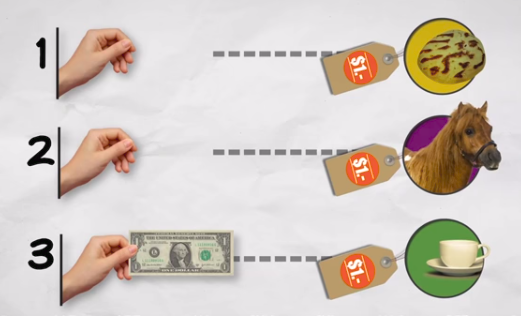
\includegraphics[width=20em]{tser_macro_01.png}

PMT'yi anlamak için bu kavramlar yeterli aslında. 1 lira para, $M$ ile
gösteriyoruz, o paranın bir senede kaç kere kullanıldığı para hızı, onu $V$
ile gösteriyoruz ki üstteki örnekte $V=3$. Poğaça, ata binmek, kahve
ekonomideki gerçek ürünler ve servisler, onlara $Y$ diyelim, ve ürün /
servislerin fiyatı ise $P$ oluyor. PMT için gerekli değişkenler bunlar. 

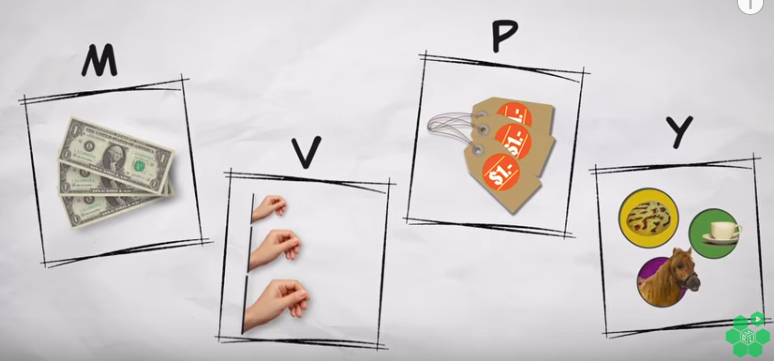
\includegraphics[width=20em]{tser_macro_02.png}

Tüm ekonomi bazında düşünürsek, $M$ para arzı (money supply) yani
ekonomideki tüm para miktarı. $V$ ürün ve servis almak için bir liranın kaç
kez kullanıldığı; bazıları parayı yastığın altına koyar onların parası
``yavaştır'', kimisi habire alışveriştedir, onların parası hızlıdır. Hız
tüm paraların hız averajı üzerinden hesaplanıyor tabii. $P$ tüm ürün ve
servislerin (yine ortalama) fiyat seviyesi. Son olarak $Y$, ekonomide
satılan tüm ürün ve servislerin miktarı, yani Gayrisafi Yurtiçi Hasıla,
GSYH (İngilizce GDP). Onun fiyat seviyesi ile çarpılmış hali Reel GSYH
(Nominal GDP), bu ekonominin ürettiği ürünlerin tüm lira bazında
toplamı. Formülün bir tarafı bu.

Formülün diğer tarafı $M$ çarpı $V$; ekonomideki tüm para miktarını o
paranın ekonomi içinde senede kaç kez döndüğü ile çarparsak bu bize, aynı
şekilde, reel GSYH'yı vermez mi? Para senede kaç kez bir ürün için birisine
verilmiş ise, bu ekonomide o kadar satış yapılmış demektir. Böylece
formülün iki tarafını elde etmiş olduk.

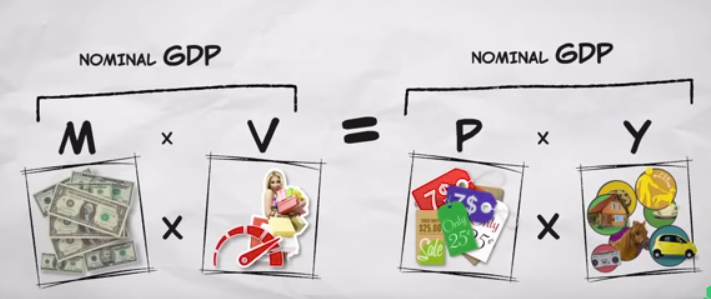
\includegraphics[width=20em]{tser_macro_03.png}

Bu formüle bir teori bile denemez, gayet bariz bir eşitlik
(identity). Formüle bir diğer bakış açısı şöyle, eldeki tüm para çarpı o
paranın kaç kez harcandığı ekonomideki tüm alıcıların yaptıklarını kapsar,
satılan her şey çarpı o şeylerin fiyatı ekonomideki tüm satıcıların
yaptıklarını kapsar. Satılan her şey tanım itibariyle alınmış olduğuna göre

$$ 
M \cdot V = P \cdot Y 
\mlabel{1}
$$

doğru olmalıdır. Tabii üstteki formüldeki değişkenlerin nasıl ölçülmesi
gerektiğiyle ilgili tartışmalar var, burada farklı yaklaşımlar
olabilir. Mesela kredi kartları para olarak $M$ içinde sayılsın mı
sayılmasın mı?

Bu tür farklılıklar bir tarafa, üstteki formül bir eşitlik olarak, ekonomi
hakkındaki fikirlerimizi organize etmesi açısından çok faydalı. Mesela
enflasyon ($P$'nin yükselmesi) sebebi nedir sorusunu formül üzerinden
cevaplayabiliriz.

Enflasyon

PMT formülünde iki tarafı $M$'ye bölelim,

$$ \frac{MV}{Y} = P$$

Bu denklem bize diyor ki eğer fiyatlar değişiyorsa bunun üç farklı sebebi
olabilir. $M$ değişiyor, $V$ değişiyor, ya da $Y$ değişiyor. Unutmayalım
fiyatlar yani $P$ (efendim domates ne kadar, pantolon, manto, ekmek
fiyatları vs) kısa sürede oldukca hızlı değisebilir, mesela bir sene içinde
fiyatların ikiye, üçe katlandığı görülmüştür. Fakat genel ekonomik
açısından biz biliyoruz ki $V,Y$ oldukca sabittir. $Y$, yani GSYH, bir sene
içinde çok, çok fazla değişmez. Bir sene içinde yüzde 10'lük çıkış muazzam
bir büyüme kabul edilir, nadir meydana gelir, ama ikiye, üçe katlanma
neredeyse hiç olmaz. Fiyatlardaki aşırı değişimi ekonomideki aşırı büyüme
ile açıklayamayız [2].

Peki paranın dolanım hızı $V$? Bu değişken 1 liranın bir sene içinde
ekonomide ortalama kaç alım yaptığını gösterir, ABD ekonomisinde bu sayı
aşağı yukarı 7 seviyesindedir. Hızı belirleyen maaşların ne sıklıkla
ödendiği, haftalık mı, aylık mı mesela, ya da bir borç senetinin, çekin
tahsil edilmesinin ne kadar zaman aldığı (ülkenin banka yapısı, bürokrasisi
ile alakalı) gibi faktörlerdir. Bunlar da yavaş değisen faktörler, bu
sebeple hız $V$ artabilir, ya da azalabilir, ama bu ABD örneğinde 8
seviyesine çıkış ya da 6 seviyesine iniş ölçüsünde olur. O zaman $P$'deki
çok büyük değişimi $V$ ile de açıklayamayız. 

Geriye ne kaldı? $M$ kaldı. Yani fiyatlardaki çıkış para arzındaki çıkışla
alakalıdır. Eğer bir ekonomide aynı miktardaki ürün ve servisin peşinde
olan para seviyesi artarsa, fiyatların yukarı çıkması gerekir. Herkesin
cebinde 100 lira olabilir, ve kahve 1 lira, sinema fiyatı 3 lira olabilir,
ama herkesin cebindeki para ikiye katlansa, ama daha fazla kahve daha fazla
sinema salonu açılmasa, kahve 2 lira, sinema 6 lira olacaktır. 

Devletler Niye Enflasyon Yaratır

Enflasyon para arzının artmasıyla ortaya çıkar, ve aslında bir tür
vergidir, çünkü zenginliği bir anlamda halktan devlete aktarır çünkü devlet
para basıp bu parayı, yeni arzı piyasada mal almak için kullanıyorsa devlet
istediğini alır, ama uzun vadede herkesin cebindeki paranın değeri düşer,
yani para basamayan halk kaybetmiş olur. Bu tür ``enflasyonist verginin''
aslında pek iyi işleyen bir yöntem olduğu söylenemez, o sebeple devletler
bu yöntemi ellerinde başka bir çare kalmadığında kullanırlar [4].

Ama yöntemin uzun vadedeki negatif tarafından önce kısa vadede olana
yakından bakalım. Aslında kısa vadede artan para arzı üretim $Y$'de artmaya
sebep olabilir. Ufak bir ekonomi düşünelim, fırıncı, terzi, ve marangoz
olsun. Diyelim devlet vergiden alacağı parayı kullanmak yerine, yeni para
basıyor ve bu parayı askerlere maaş olarak veriyor. Askerler alışverişe
çıktıklarında, giysi, ekmek ve aldıklarında ilk başta mesela fırıncı çok
mutlu olur, ekmeğini satacak yeni talep ortaya çıkmıştır. Fırıncı yeni
talebi karşılamak için daha uzun saatler çalışır, daha fazla eleman ise
alır, talep artınca fiyatları da arttırabilir. Fırıncı ``oh ne güzel, artan
ekmek fiyatları ve satışı sayesinde kazandığım ek para ile daha fazla giysi
ve sandalye alabilirim''. Fakat askerler marangozdan, ve terziden de aynı
alışveriş yapmaktadırlar, onların da fiyatları artmaktadır. Fırıncı yeni
parasıyla pantolon almak için terziye gittiğinde neredeyse kazandığı ek
para kadar fiyatların artmış olduğunu görür, yani alım gücü aynı
kalmıştır. Parasının değeri düşmüştür.

Fakat devletin işi de bozulacaktır, çünkü onlar için de fiyatlar artmıştır,
para basıp aynı malları aldırmak istediğinde yeni fiyatlarla aynı alım için
daha fazla para basmak zorundadır. Basarsa bu hikaye aynı şekilde devam
eder, para değerini kaybetmeyi sürdürür, ayrıca bir süre sonra esnaf
uyanır, fiyat artışını öngörmeye başlarlar / olacağını bilirler, ve artık
``yeni talebi'' tatmin etmek için daha fazla üretmezler.

Kısa ve uzun vade ile kasettiğimiz budur. Para arzını arttırmak başta
üretimi arttırabilir, ama devletler bu numarayı istismar edebilirler,
mesela Zimbabve'de seçim kazanmak için Mugabe'nin yaptığı gibi, ve sonuçlar
her zaman kötü biter. Çünkü kısa vadede üretim artışı ardından esas artış
fiyatlara yansır ve üretim aynı seviyeye düşer, diğer yandan eğer devlet
enflasyonu çok yukarıdan azaltmak istiyorsa para arzında daralma yaratması
gerekince ilk başta üretimde düşüş olacaktır, ki bu ekonomik durulma, hatta
kriz demektir, ta ki arzdaki daralma fiyatlara yansıyıncaya kadar. Yani
enflasyonist numara başta işe biraz yarayabilir, ardından işe yaramamaya
başlar, ve kriz kaçınilmaz hale gelir. Bu noktada enflasyonun azalması
ekonomide yavaşlama, işsizlik artışına sebep olur. 

Bu sebeple bazıları enflasyonu bir uyuşturucuya benzetir. İlk başta
``uçurabilir'' ama bünye alıştıkça aynı uçuşu sağlamak için daha ve daha
fazla ilaç gerekir, öyle ki bir süre sonra kişi normal olmak için bile
ilaca ihtiyaç duyar, ve ardından ilaç kullanımı durdurulunca bir süre
``yokluk krizi (withdrawal)'' ile hasta şok yaşar, ardından acılı bir süreç
sonrası normale dönülür. ABD'de 70'li yıllarda olan buydu, 70'ler boyunca
enflasyon arttı, arttı, ama 70'ler sonunda artık işe yaramıyordu, işsizlik
düşmüyordu. Bu noktada stagflasyon denen şey ortaya çıktı yani hem
enflasyon hem işsizliğin aynı anda olduğu durum. 80'lı yıllar başında
Reagan başkan olunca enflasyon düştü, ama bunun bedeli 81/82 yıllarındaki
kriz oldu.

Para Nedir 

Biraz önce devletin ``para bastığından'' bahsettik, para basılıp askerlere
veriliyordu. Fakat [3]'e göre para arzının esas odağı aslında bankaların
işyerlerine ve bazen özel kişilere verdiği {\em kredidir} çünkü banka borç
verirken para basar. 

Pek çok kişi bu bilgiden habersizdir. Bir şirket bankaya gidip borç
istediğinde, borç verilirse banka hiç yoktan para yaratmaktadır, ve bu
``yeni parayı'' borç isteyene vermektedir. Bu tabii ki para arzında
genişlemeye sebep olacaktır, ve (1) denklemi üzerinden ekonomi
etkilenir. Bu sebeple arz hakkında her türlü hesap ekonomideki borç
miktarını göz önüne almak zorundadır [3]. 2008 krizine kadar pek çok
kişinin bilmediği bu durum yakın zamanda İngiliz ve Alman Merkez Bankaları
tarafından kabul edildi. Evet bankalar hiç yoktan para yaratıyorlar. Yani
bankaların ``özel kişilerin mevduatını borç olarak verdiği'' doğru
değildir. Bankaların borç vermek mevduata ihtiyacı yoktur, parayı basar ve
verir [5].

Eski para tanımını kullananlar bu sebeple Japonya, ABD'de 80'li yıllarda
ortaya çıkan hız yavaşlama durumunu açıklayamadılar. (1) formülünde hızın
çoğunlukla değişmediğini söylemiştik, yani 

$$ V = PY / M$$

sabit seviyede olmalıydı. Fakat alttaki grafikte hızın

\begin{minted}[fontsize=\footnotesize]{python}
import pandas as pd
df = pd.read_csv('money.csv',parse_dates=['DATE'])
df = df.set_index('DATE')
df = df[['m2cd','gdp']]
df = df.ix[df.index > '1960-01-01']
df = df.ix[df.index < '2010-01-01']
df = df.dropna(axis=0)
df['vel1'] = df.gdp / df.m2cd
df.vel1.plot(ylim=[0.0,3.0])
plt.savefig('tser_macro_04.png')
\end{minted}

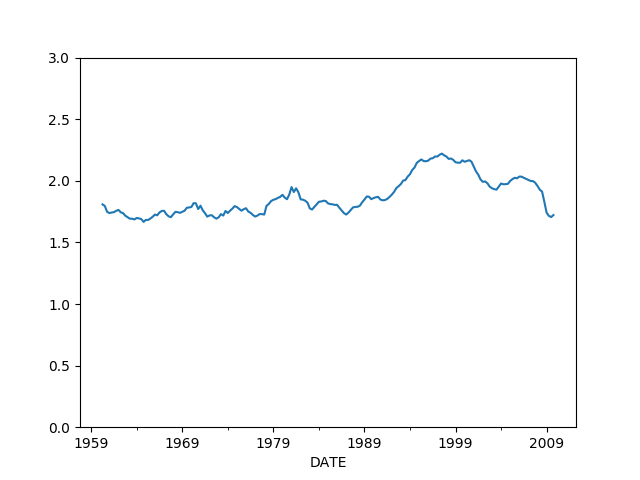
\includegraphics[width=20em]{tser_macro_04.png}

sabit olmadığını görüyoruz. Niye? Sebep yanlış seçilen $M$. Yani aslında
hız yavaşlaması olmadı, $M$ ölçütü doğru kullanılmadığı için hız
yavaşlıyormuş gibi durdu. Üstteki grafik ve benzerleri için ekonomistler
bir para arzı ölçütü olan M0, M1, M2, vs. gibi rakamları kullanıyorlar. Bu
ölçütler banka mevduatlarına, merkez bankalarının ``bastım'' dediği para
miktarı gibi toplamları baz alıyor. Çoğunlukla kullanılan M2, üstteki
grafikte onu kullandık. Fakat para arzı aslında direk bankların verdiği
kredi ile alakalı. O zaman doğru $M$ için krediye bakmak lazım. Fakat
hikayenin devamı da var.

(1) formülüne bakmanın bir diğer yolu daha var. Eğer ekonomideki kredi
$M$'yi (yani artık biliyoruz ki parayı) aşırı arttırırsam, ve bu artış GSYH
artışından daha fazla olursa ne olur?  Enflasyon. Enflasyonun pek çok
çeşidi var; ev fiyatlarının, borsanın aşırı artması da, yani balonlar da
bir tür enflasyondur. Fakat bu tür ürünlerin GSYH ile ölçülen ürünlerden
farklı olduğunu kestirmek mümkün. O zaman, eğer reel sektöre, gerçek
büyümeye odaklanmak istiyorsak, $M$ için kredi kullanırken iki türlü kredi
olduğunu görmek gerekir, biri üretime giden ``iyi'' kredi, diğeri emlak,
spekülasyona giden ``kötü'' kredi. Finans sektörüne giden her türlü kredi
balona gider, enflasyon yaratır. İnşaat, emlak sektörü de aynı
şekilde. Tabii spekülasyon olmasın (o da lazım), inşaatçılar borç almasın
demiyoruz. Sadece bu borçlanma ``para basarak olamaz'' diyoruz, yani bu tür
akvitiler için para arzı genişleyemez. ABD 2008 krizinde olan aynen buydu,
regülasyonları gevşemiş bankalar spekülatif oyunlar için para bastılar,
balon oluştu ve patladı. Hıza dönersek, o zaman ekonomideki finans dışı tüm
kredileri alıp, ondan emlak kredilerini çıkartırsak, ve bu ``iyi'' $M$
üzerinden hızı grafiklersek,

\begin{minted}[fontsize=\footnotesize]{python}
df3 = pd.read_csv('money.csv',parse_dates=['DATE'])
df3 = df3.set_index('DATE')
df3 = df3.ix[df3.index > '1960-01-01']
df3 = df3.ix[df3.index < '2010-01-01']
df3 = df3[['m2cd','gdp','nonfincred','realest']]
df3 = df3.resample("A", how='sum') 
df3['vel2'] = df3.gdp / (df3.nonfincred-df3.realest)
df3.vel2.plot(ylim=[0.0,3.0])
plt.savefig('tser_macro_05.png')
\end{minted}

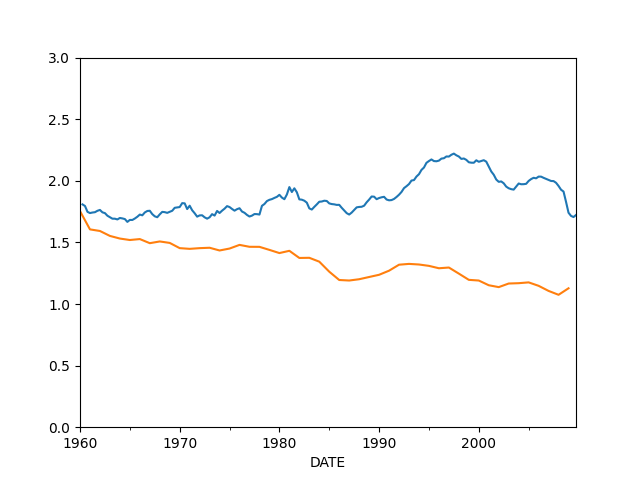
\includegraphics[width=20em]{tser_macro_05.png}

Bu hızın daha stabil olduğunu görüyoruz. Verileri farklı şekilde toplamak
mümkün, bizim ABD için seçtiğimiz yöntem [3] yaklaşımından biraz daha
farklı, [3, sf. 204] Japonya için de daha da stabil bir eğri bulmuş. 

Werner [3, sf. 185] daha da ileri giderek GSYH üretecek ``iyi'' ticaret,
mal ve servis alımını spekülatif, ``kötü'' üretimden formül bazında da
ayırıyor, $M = M_R + M_F$ diyor, ki $M_R$ gerçek ekonomi $M_F$ spekülatif
ekonomidir, ardından,

$$ M_RV_R = P_RQ_R = P_RY$$

$$ M_FV_F = P_FQ_F$$

Bu seçimin faydası GSYH ile uğraşırken verisel olarak onunla alakalı olan
diğer verileri net olarak belirleyebilmek. Eğer GSYH verisine bakıyorsak o
zaman onu üretecek kredi türlerine, onların verisine bakmak gerekir.

Merkez Bankası Faizleri Büyümeyi Etkiler mi?

Neoklasik ekonomiye göre düşürülen faizler büyümeyi teşvik eder,
yükseltilen faizler durgunluğa sebep olur. Fakat veriye bakınca bunun doğru
olmadığını görüyoruz [7]. Test etmek için merkez bankası faizleri ve büyüme
rakamlarını indiriyoruz, ve üzerinde Granger sebep olma (causality) testi
uyguluyoruz. Bu test iki zaman serisini alır ve ikincisinin birincisine
sebep olup olmadığını ölçer. Sıfır hipotez olmadığıdır, o zaman hipotez
reddedilirse bunu sebep olma yönünde güçlü kanıt olarak alabiliriz. Altta
ilk önce faizlerin büyüme üzerinde etkisi, sonra büyümenin faizler üzerinde
etkisine bakıyoruz.

\begin{minted}[fontsize=\footnotesize]{python}
import statsmodels.tsa.stattools as t
import pandas as pd

df = pd.read_csv('rates.csv',parse_dates=['DATE'])
df = df.set_index('DATE')
df = df.resample('AS').last()
df['gdpinc'] = df.gdp.pct_change()*100.0
df = df.dropna(axis=0)
res = t.grangercausalitytests(df[['gdpinc','shortrate']],maxlag=2)
res = t.grangercausalitytests(df[['shortrate','gdpinc']],maxlag=2)
\end{minted}

\begin{verbatim}

Granger Causality
('number of lags (no zero)', 1)
ssr based F test:         F=0.0062  , p=0.9378  , df_denom=43, df_num=1
ssr based chi2 test:   chi2=0.0066  , p=0.9353  , df=1
likelihood ratio test: chi2=0.0066  , p=0.9353  , df=1
parameter F test:         F=0.0062  , p=0.9378  , df_denom=43, df_num=1

Granger Causality
('number of lags (no zero)', 2)
ssr based F test:         F=0.2645  , p=0.7689  , df_denom=40, df_num=2
ssr based chi2 test:   chi2=0.5952  , p=0.7426  , df=2
likelihood ratio test: chi2=0.5913  , p=0.7440  , df=2
parameter F test:         F=0.2645  , p=0.7689  , df_denom=40, df_num=2

Granger Causality
('number of lags (no zero)', 1)
ssr based F test:         F=14.0199 , p=0.0005  , df_denom=43, df_num=1
ssr based chi2 test:   chi2=14.9980 , p=0.0001  , df=1
likelihood ratio test: chi2=12.9812 , p=0.0003  , df=1
parameter F test:         F=14.0199 , p=0.0005  , df_denom=43, df_num=1

Granger Causality
('number of lags (no zero)', 2)
ssr based F test:         F=9.2853  , p=0.0005  , df_denom=40, df_num=2
ssr based chi2 test:   chi2=20.8919 , p=0.0000  , df=2
likelihood ratio test: chi2=17.1609 , p=0.0002  , df=2
parameter F test:         F=9.2853  , p=0.0005  , df_denom=40, df_num=2
\end{verbatim}

Sonuca göre büyüme faizleri etkiliyor, ters yönde bir etki söz konusu
değil. Altta etkinin korelasyonuna bakıyoruz,

\begin{minted}[fontsize=\footnotesize]{python}
import scipy.stats as stats
df['gdpinc1'] = df.gdpinc.shift(1)
df2 = df.dropna(axis=0)
print stats.pearsonr(df2.shortrate, df2.gdpinc1)
\end{minted}

\begin{verbatim}
(0.75710287451587455, 1.1393168782627738e-09)
\end{verbatim}

Etkinin korelasyonu pozitif, yani büyüme faiz arttırımına, küçülme faiz
düşürülmesine sebep oluyor.

Madem durum böyle niye ekonomistler sürekli faizlerden bahsediyorlar? [3]'e
göre sebep politik. Merkez ve ticari bankalar esas manivelanın kredi
yönlendirmesi olduğunu halktan saklamak istiyorlar, çünkü bu çok güçlü bir
araç, bu aracı politikacılardan uzak tutmak istiyorlar ve kendi
ajandalarını takip ediyorlar. Mesela Japonya'nın 90'li yılllarda başlayan
ve bitmek bilmeyen krizi aslında kredi daralması ile Japon merkez
bankasının yarattığı bir krizdir, ve bu sırada sürekli ``yapısal reform''
sözleri söylenmiştir, amaç Japonya'nın daha ABD'ye benzeyen bir ekonomi
olmasını sağlamaktır. AB'de çevre ülkelerde meydana gelen kriz aslında suni
bir krizdir, Avrupa Merkez Bankası bu ülkelere krediyi aşırı arttırmıştır,
büyümeyi çok çok aşan bu para doğal olarak enflasyona, emlak piyasasına
akmıştır. Amaç kriz ortamında finansal bağlantıları merkezi haline
getirmek, AB projesini ilerletmektir.

Teorik olarak neoklasik ekonominin faizleri sevmesinin sebebi olmayan yerde
sürekli denge arayan teorileridir. Bu teorilere göre arz/talep vardır, ve
paraya olan arz ve talep ``paranın fiyatı'' olan faizi ortaya
çıkarır. Fakat ticari bankalar parayı hiç yoktan yaratırlar, ve bu paraya
pratikte sonsuz talep vardır (pek çok kişi kredi almak ister), eğer piyasa
şartları devreye girseydi faizlerin müthiş fazla olması gerekirdi. Bu
olamayınca, kredi piyasasında arz/talebin işlemeyeceği
görülecektir. Arz/talep işlemeyince çok olan bir şey (borç isteği) ile az
alınabilecek şey (kredi) ilişkisinde, yani az miktar ile çok miktar
arasında her zaman az olan kuralları koyar, ya da arzın bir nevi ``karneye
bağlandığı (rationed)'' da söylenebilir, yani kredi sağlayan istediği
fiyatı, kendisine uygun ölçüde, belli sayıdaki müşteriye ama çok aşırı
olmayacak şekilde belirler.

Karneye bağlama kavramından bahsedilmeye başlanınca bazı sosyal
tercihlerin yapılması gerektiği, yapılacağı bir durum ortaya çıkar, devlet
ya da diğer iç odaklar devreye girebilir, kredi hangi yöne sağlanacak,
hangi amaçlar için yaratılacaktır? Bu noktada halkın geleceği
gözetilecektir, en azından böyle olacağı umulur.

Kriz zamanında devletin harcamaları arttırması büyümeye yardım eder mi? 

Cevap hayır [3, sf. 249], alttaki test kamu harcamasının özel sektörü
yerinden etmesi (crowding-out) teorisini doğruluyor. Eğer devlet bono ile
borçlanırsa ve onu harcarsa, bir cepten alınan para diğerine konulmuş olur,
para arzında değişim olmaz. [3]'e göre para = kredi, eğer spekülasyon
olmayan ``GSYH üreten'' aktivitelere para arzı (kredi) artmamışsa büyüme
olmaz.

Formül üzerinde görmek için ana denklem ile başlayalım, ama onun gerçek
sektörü etkileyen kısmı ile ilgilenelim,

$$ 
P_R Y = V_R C_R 
\mlabel{4}
$$

ki $C_R$ reel sektöre giden kredi (para arzı). Farklılıklara bakarsak, 

$$ 
\Delta (P_R Y) = V_R \Delta C_R 
\mlabel{2}
$$

$P_rY$ reel GSYH. Farklılık operatörünü $V_R$ üzerinde uygulamadık çünkü
hızı sabit kabul ettik. Şimdi $P_rY$'yi ayırmak için alttaki değişkenleri
tanımlayalım,

$c$ reel tüketim (nominal consumption)

$g$ reel devlet giderleri (nominal government expenditure)

$i$ reel yatırım (nominal investment)

$nx$ reel net ihracat (nominal net exports)

Ve

$$ 
\Delta (P_RY) = \Delta c + \Delta i + \Delta g + \Delta nx 
\mlabel{3}
$$ 

olarak ayırıyoruz. (2)'yi üstteki denkleme sokunca, 

$$ \Delta (c +  i +  nx) = V_R\Delta C_R - \Delta g$$

Bu eşitliğin sol tarafı talepteki artışı temsil ediyor. Üstteki denklem
ilginç bir şey söylüyor aslında, banka sisteminin ürettiği kredinin sabit
olduğu şartta devlet harcamaları $g$'deki her büyüme eşit ölçüde talep
azalmasına sebep olmalı; çünkü $\Delta g$'nin katsayısı -1.``Aynı olduğu
şartı'' faraziyesini test edebiliriz, çünkü bir regresyon uyguladığımızda
rapor edilen katsayılar aynen bu faraziyeye göre hesaplanırlar. 

Şimdi sayısal test için gerekli denklemi kuralım. Farklılıkta hız
kavramına gerek yok, ayrıca yüzdesel artım, azalım ile konuşmak
istiyoruz. Log'ların farklılıklarının kabaca yüzde artışı olduğunu
biliyoruz, log'u alınmış değişkenleri küçük harfi ile temsil edersek, 

$$ \Delta p_R + \Delta y = \Delta c_R$$

Şimdi üstteki denklemdeki zaman indislerini göz önüne alalım. Bir periyotta
yaratılan kredi bir sonraki periyottaki büyümeyi etkiler, o zaman üstteki
denklem,

$$ \Delta p_{Rt} + \Delta y_{t} = \Delta c_{Rt-1}$$

haline gelir. Ya da 

$$ \Delta GDP_t = \Delta C_{Rt-1}$$

Her iki tarafa $\Delta GDP_{t-1}$ ekleyelim,

$$ \Delta GDP_t + \Delta GDP_{t-1} = \Delta C_{Rt-1} + \Delta GDP_{t-1} $$

İki üsttekini yerine koyalım,

$$ \Delta GDP_t + \Delta GDP_{t-1} = \Delta C_{Rt-1} + \Delta C_{Rt-2}  $$

$$ \Delta GDP_t = - \Delta GDP_{t-1} + \Delta C_{Rt-1} + \Delta C_{Rt-2}  $$

Şimdi üstteki formülü test etmek için regresyon katsayıları verelim,

$$ \Delta GDP_t = 
\alpha + \beta_1 \Delta GDP_{t-1} + 
\gamma_0 \Delta C_{Rt-1} + \gamma_3 \Delta C_{Rt-2} + \epsilon_t 
$$

Sol kısmı (3)'e bakarak açıyoruz ve $\Delta g$'yi sağ tarafa geçiriyoruz,

$$ 
\Delta (c_t + i_t + nx_t) = 
\alpha + \beta_0 \Delta g_t + \beta_1 \Delta GDP_{t-1} + 
\gamma_0 \Delta C_{Rt-1} + \gamma_3 \Delta C_{Rt-2} + \epsilon_t 
$$

O zaman biraz önce bahsedilen yerinden etme teorisi doğruysa devlet
harcamalarındaki değişimin katsayısının eksi bir olduğunu veriden katsayı
hesapladığımızda görmemiz lazım. Regresyonu kuralım,

\begin{minted}[fontsize=\footnotesize]{python}
import pandas as pd
df = pd.read_csv('crowd.csv',parse_dates=True)
df = df.dropna(axis=0)
df = df.set_index('DATE')
df['gdp'] = df.gdp / 1000.0
df['govexp'] = (df['gov1exp'] + df['gov2exp']) / 1000.0
df['lhs'] = (df.consump + df.invest + df.netexp).pct_change() 
df['dgt'] = df.govexp.pct_change() 
#df['dcrt'] = (df.nonfinloan - df.constructloan).diff() / 1000.0
df['dcrt'] = (df.nonfinloan).diff() / 1000.0
df['dcrt1'] = df.dcrt.shift(1)
df['dcrt2'] = df.dcrt.shift(2)
df['dcrt3'] = df.dcrt.shift(3)
df['dgdpt'] = df.gdp.pct_change()
df['dgdpt1'] = df.dgdpt.shift(1)
df['dgdpt2'] = df.dgdpt.shift(2)
df = df.dropna(axis=0)

import statsmodels.formula.api as smf
results = smf.ols('lhs ~ dgt +  dgdpt1 + dcrt1  + dcrt2 ', data=df).fit()
print results.summary()
\end{minted}

\begin{verbatim}
                            OLS Regression Results                            
==============================================================================
Dep. Variable:                    lhs   R-squared:                       0.106
Model:                            OLS   Adj. R-squared:                  0.086
Method:                 Least Squares   F-statistic:                     5.346
Date:                Sun, 20 May 2018   Prob (F-statistic):           0.000432
Time:                        22:57:54   Log-Likelihood:                 358.03
No. Observations:                 185   AIC:                            -706.1
Df Residuals:                     180   BIC:                            -690.0
Df Model:                           4                                         
Covariance Type:            nonrobust                                         
==============================================================================
                 coef    std err          t      P>|t|      [95.0% Conf. Int.]
------------------------------------------------------------------------------
Intercept      0.0138      0.006      2.185      0.030         0.001     0.026
dgt           -0.5671      0.183     -3.101      0.002        -0.928    -0.206
dgdpt1         0.5867      0.271      2.165      0.032         0.052     1.122
dcrt1          0.0375      0.034      1.101      0.272        -0.030     0.105
dcrt2         -0.0754      0.034     -2.208      0.028        -0.143    -0.008
==============================================================================
Omnibus:                        6.056   Durbin-Watson:                   2.107
Prob(Omnibus):                  0.048   Jarque-Bera (JB):                7.103
Skew:                          -0.245   Prob(JB):                       0.0287
Kurtosis:                       3.825   Cond. No.                         108.
==============================================================================

Warnings:
[1] Standard Errors assume that the covariance matrix of the errors is correctly specified.
\end{verbatim}

$\Delta g$ katsayısı -0.56 çıktı. Veri toplamadaki değişimle alakalı
olabilir, fakat [3]'te Japonya verisi için Werner tam -1 buldu. Katsayı
istatistiki olarak önemli, ve genel model uyumu $R^2$ 10 civarında. Fena
sayılmaz. Yani devletin harcadığı her dolar aşağı yukarı aynı miktarda
doları (ya da lirayı) yerinden ediyor. Büyümeye yardım etmiyor.

Böylece ana kavramları görmüş olduk. Sorulabilir ki büyüme için teknolojiye
yatırım, eğitim, vs. sözleri söylenir. Bunlar neyi arttırır? Bu
bahsedilenler aslında ekonomik kapasiteyi arttırırlar (hatta kapasite
arttırımı için iyi bir yöntem [14] yazısında bulunabilir). İyi seçimler
yapılırsa kapasite diyelim yüzde 2'den yüzde 5'e artsın. Sonra yapılması
gereken bu kapasiteye gerekli krediyi sağlamak. Bu arada eğer kredi büyüme
kapasitesini karşılayacak kadar sağlanmazsa deflasyon ortaya çıkar [8],
Japonya gerçek ürünlerde bunu da yaşadı.  Deflasyon sebebi (4) formülünün
basit bir uygulaması sadece, eğer büyüme kapasitesi artmış yani daha fazla
$P$ elde ediyorsak ama eşitliğin sol tarafında kredi yerinden oynanamışsa
bu fiyatlar $P$ üzerinde aşağı doğru baskı yapar.

Eğer para arzı büyümeyi aşarsa enflasyon ortaya çıkar. Spekülasyon,
tüketime giden kredi enflasyona gider.



Kaynaklar

[1] Marginal Revolution University, {\em Quantity Theory of Money}, 
    \url{https://youtu.be/q59tZKP0HME}

[2] Marginal Revolution University, {\em Causes of Inflation}, 
    \url{https://youtu.be/gi7jx5IJtik}

[3] Werner, {\em New Paradigm in Macroeconomics}

[4] Marginal Revolution University, {\em Why Governments Create Inflation}, 
    \url{https://youtu.be/E6A_WpUY2LI}

[5] {\em Money as Debt}, 
    \url{https://www.youtube.com/watch?v=2nBPN-MKefA}

[6] Wikipedia, {\em Money supply}, 
    \url{https://en.wikipedia.org/wiki/Money_supply}

[7] {\em Reconsidering Monetary Policy: An Empirical Examination of the Relationship Between Interest Rates and Nominal GDP Growth in the U.S., U.K., Germany and Japan},
    \url{https://www.sciencedirect.com/science/article/pii/S0921800916307510}

[8] {\em Applying the Quantity Theory of Credit: The role of the ECB in the propagation of the European financial and sovereign debt crisis and the policy implications}, 
   \url{http://www2.euromemorandum.eu/uploads/werner_qtc_ecb_and_policy.pdf}

[13], Werner, {\em The Quantity Theory of Credit and Some of its Applications}, 
     \url{https://www.postkeynesian.net/downloads/Werner/RW301012PPT.pdf}

[14] Bayramlı, Lineer Cebir, {\em Ülkelerin Ekonomik  Kapasiteleri}



\end{document}
